\documentclass{article}
\usepackage[english]{babel}
\usepackage[T1]{fontenc}
\usepackage{wrapfig}
\usepackage{lscape}
\usepackage{rotating}
\usepackage{graphicx}
\usepackage{listings}
\usepackage{amsmath}
\usepackage{mathtools}
\usepackage{amsfonts}
\usepackage{hyperref}
\usepackage{array}
\usepackage{booktabs}
\usepackage{multicol}
\usepackage{biblatex}
\addbibresource{refs.bib}

\title{Chips Operational Semantics}
\author{Anna <3}
\date{\today}

% Source - https://tex.stackexchange.com/a/136050
% Posted by petermeissner, modified by community. See post 'Timeline' for change history
% Retrieved 2026-05-06, License - CC BY-SA 3.0

\newenvironment{myitemize}
{ \begin{itemize}
    \setlength{\itemsep}{0pt}
    \setlength{\parskip}{0pt}
    \setlength{\parsep}{0pt}     }
{ \end{itemize}                  } 



\newcommand{\eqdef}{\stackrel{\mathclap{\normalfont\mbox{\footnotesize def}}}{=}}

\newcommand{\aoverb}[2]{\stackrel{\mathclap{\footnotesize #1}}{#2}}
\newcommand{\s}{\hspace{1em}}

\newcommand{\mprod}{\text{ \textbf{m} }}

% Source - https://tex.stackexchange.com/a/371469
% Posted by Moriambar, modified by community. See post 'Timeline' for change history
% Retrieved 2026-05-29, License - CC BY-SA 4.0
\newcommand{\myrule}{\par\noindent\rule[-1pt]{0.5\textwidth}{0.4pt}\\}

\begin{document}

\maketitle

\section*{Introduction}
Chips permits its users to describe models of systems executing programs. Therefore, it does not only allow to design algorithms, but also cares about notions such as ``program embedding'', ``dataflows'' or ``device interconnections''. The simultaneous need to describe both algorithms and devices implies a syntax that mixes elements of both imperative and declarative (synchronous) paradigms. Additionally, the coordination of many components in a single system requires a new kind of (collective) primitives that allows the specification of the data evolution when spread or collected among crowds of devices, where local information matters.
This document describes a formal interpretation for the models the Chips language allows to implement. Thank to this description, it becomes possible to draw proofs or formal property definitions for any given Chips model at a system-wide abstraction level.
Section~\ref{overview} explores briefly the main system description concepts of the language. Then, Section~\ref{osemantic} precises formally such concepts to demonstrate its ability to implement the concept of Hierarchical Control Motifs for complex systems design.

\section{Overview of Chips modeling concepts}\label{overview}

Chips is a language for defining Cyber-Physical Systems (CPS) putting the emphasis on the compositional aspect of each functionnalities. The broad definition of ``systems'' that we adopt can be summed up as ``a set of \emph{components} in interaction that together \emph{provide a service}''. 
In Chips, the notion of providing a service leads to the concept of \emph{function}, while the notion of components is embodied by the concept of \emph{node} embedding such functions. To permit the coordination of functions accross nodes, Chips introduces the concept of user defined \emph{collective primitives}.
These three ideas are detailed in the following subsections. 

\subsection{Functions}\label{functions}

Functions are the abstraction chosen to represent running processes in a Chips model. When defining them, one must specify:
\begin{itemize}
    \item a set of typed input variables and their potential default values,
    \item an initializing process that defines inner state variables and their potential default values,
    \item an updating process that defines the evolution of the inner state variables according to the values of input variables, and
    \item a set of named and type-deduced output expressions.
\end{itemize}

To showcase the syntax of Chips applied to the definition of a function, Figure~\ref{logical} presents the definition of a function that computes simultaneously the sum and the product of its input.

\begin{figure}
    \centering
    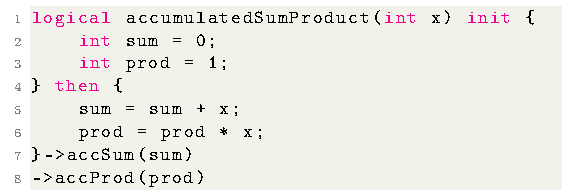
\includegraphics{imgs/functionexamplesimple.pdf}
    \caption{Definition of a Chips function}\label{logical}
\end{figure}

Broadly speaking, when instanciated, a function applies its initializing protocol (the \emph{init} section). Then, it applies its updating process (the \emph{then} section) everytime all its input variables are updated exactly once. If an input variable has a default value, Chips considers it has already been updated once at the initialization of the model. 
Therefore, when connecting input and outputs of functions, one must care about the presence/absence of default values for inputs of components to correctly understand the way dataflow evolve or why some compositions may lead to delayed system deadlock, as shown in figure~\ref{deadlocks}.

\begin{figure}
    \centering
    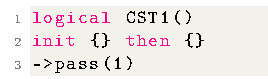
\includegraphics[width=0.3\columnwidth]{imgs/CST1.pdf}
    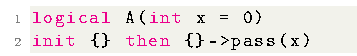
\includegraphics[width=0.3\columnwidth]{imgs/A.pdf}
    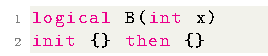
\includegraphics[width=0.3\columnwidth]{imgs/B.pdf}
    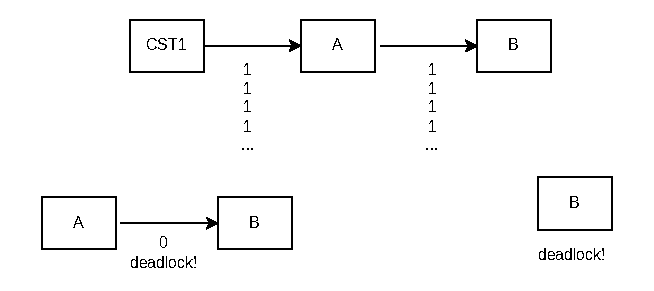
\includegraphics[width=\columnwidth]{imgs/chips_deadlocks.pdf}
    \caption{Presence or absence of deadlocks for sets of functions defined with or without default values for their input.}\label{deadlocks}
\end{figure}

From the model composition perspective, they can be seen as black boxes providing an interface being their set of inputs and their set of outputs. A functional block with all its inputs having a default value is able to \emph{trigger} the components depending on it once because it has all the required information to compute its \emph{then} section once. Remark that functional blocks with no input parameter are always able to compute the content of their \emph{then} section because such computation does not depend on pre-computed data. So they never can be a source of deadlock for the system. 

The composition of functional blocks leads to the creation of a directed graph, which we will call the \emph{functional graph}. The vertices are the functions and the edges are the input/output linkage between the functions. The presence of loops in the graph signifies that at least a part of the designed system retro-acts on itself. Just as the wheels of a vapor train, all functions run their \emph{then} sections altogether, one function giving the pace for the next ones. Therefore, no clock is explicitly defined for the systems. The execution of the \emph{then} section of any component can serve as an implicit clock tick.

The graph formalism applied to the functional dependency of the model elements allow to perform early checking of properties of the model before it is instanciated on a real system.

\subsection{Nodes}

Nodes are an abstraction of the Chips models that represent locations. If two events happen in different places, a model accounting such difference will make each event interact with different nodes. In the context of complex CPSs, nodes can be instanciated to represent a physical separation of processes, or a logical separation for processes that are based on distinct sets of information. Nonetheless, these two use cases of nodes feature common characteristics:
\begin{itemize}
    \item they are responsible of data related to the location they represent, and
    \item they provide a set of typed labels to specify their possibility to exchange data with other nodes.
\end{itemize}

In the case of a node modeling a virtual location, that node is defined as a Chips \emph{object}. An object definition simply gets described as a set of instructions comprising the declaration of \emph{contextual variables} (using the keyword ``ctx'' as in line 3 of Figure~\ref{object}) and the declaration of \emph{channels} (by writing an instruction of two identifiers as in line 4 and 5). Imperative code instructions can also be used in such definitions to define default values of contextual values, but such details go beyond the scope of the system level coordination mechanisms studied in this document.  

\begin{figure}
    \centering
    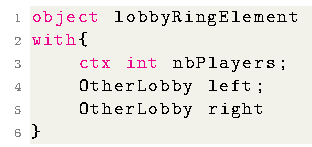
\includegraphics[width=0.5\columnwidth]{imgs/lobbyring.pdf}
    \caption{An object (virtual location) representing an instance of a lobby for a multiplayer server model}\label{object}
\end{figure}

Chips functions can be \emph{embedded} in nodes. When it is the case, functions can refer to contextual variables as if they were defined in their own scope. To do so, we use the \verb'ctx.<ctx_variable_name>' notation in the code sections of the components using it.

Channels are the Chips way to specify how different nodes are connectable together. They feature a \emph{channel type} being an arbitrarily named type (excluding Chips keywords). During the evaluation of the system description section, these channel types allow to ensure the components connected together are compatible.

The definition of a node is orthogonal to the definition of a function, therefore, Chips provides the mean to define functions that are inherently attached to a node. Such concept is particularly relevant when designing components that emulate the physical behavior of a device. This is why such components are defined with the keyword \emph{physical}. The \emph{object} keyword allows to design a node as an abstraction for regrouping functions under a single component with shared contextual values. Such objects cannot exist on their own, they must be instanciated as embedded by physical nodes of a Chips model.

This embedding concept gives rise to a second kind of directed graph, adjacent to the \emph{functional graph} of the previous section. We will call this graph the \emph{mapping graph}. Its vertices can either be functions or nodes, and the edges represent the belonging of a function or a node to another node. Such graph has to be acyclic as an object cannot embed itself.

The graph formalism applied to the concept of embedding allows, just like for the functional graph, to perform early checking of properties of a system, but also to construct upon it the last specificity of Chips, \emph{collective primitives}.

\subsection{Collective primitives}

With the current set of model elements described for Chips, it is possible to define two things:
\begin{itemize}
    \item the evolution of signals among components of a system and
    \item the embedding relation of processes with the parts of system that contain them.
\end{itemize}

However, when designing large systems, the declination of the signals when they have to be spread among many component can become hard, in particular when accounting local information. The current tools available would require to either duplicate our functional blocks as many times as there are different configurations for receiving the data. The same problem is true when it comes to aggregating signals.

Our proposition with the Chips language is to let the programmer design a new kind of operator to describe the way data is modified by the context in which it is spread or collected. Hence the concepts of \emph{spread} and \emph{collect} collective function definitions.

They are comparable to the idea of \emph{Streams} in the java language, except that, instead of processing the evolution of an accumulated value across logical time, they process the evolution of an accumulated value across logical space (i.e.~the stream is updated when it reaches a new components). Such operation is sensitive to the architecture of the model formed, so it cares about the path data takes to go from one node to another. Since the interconnection between nodes is specified by plugging node \emph{channels} together, collective functions also make use of the channels defined to specify data propagation.

A collective function definition is composed of:
\begin{itemize}
    \item a direction keyword (\emph{spread} or \emph{collect}),
    \item a default accumulator definition,
    \item a support node reference,
    \item a stream update code section,
    \item a \emph{target} output expression,
    \item a specification of updated accumulator for each channel of the referenced node.
\end{itemize}

The direction \emph{spread} signify that information transmitted originates from a single component and gets propagated to many others. The direction \emph{collect} signify the information originates from many components and get merged together to become the input of a single one.
The default accumulator definition respects the same rules of the regular Chips function input parameters definition, except that each variable declared as a parameter \textbf{must} be provided with a default value.

To reference a support node, simply use the name of the node definition to use as support. This allows to compute when the stream update process is relevant to apply, thus respecting the \emph{mapping graph} for the propagation of data.

The target output expression must be of the type of the input of the Chips function that will receive the propagated data. It is annoted with the \texttt{@} symbol.

Updated accumulators must be specified for each channel that is defined for the type of node that the collective function references.
\begin{itemize}
    \item For \emph{spread} operations, all of the channel accumulators but the one that provided the input accumulator to the collective function will be used.
    \item For \emph{collect} operations, only the channel accumulator that goes in the direction of the collecting component will be used.
\end{itemize}

Chips provides a \emph{default} accumulator keyword to define the updated accumulator expression for all the channels that do not have a specification yet.
In the context of collective functions, the set of instructions for the stream update code section is the same as the one from regular functions. However, the semantics of expressions in this context differs in two different ways:
\begin{itemize}
    \item each datatype is enhanced with a new value (represented by the keyword \emph{stop})
    \item some new variables are available by default (the \emph{input} and channel related and variables).
\end{itemize}

\subsubsection{Semantics for \emph{stop}}
The \emph{stop} value is to signify that a variable must not be processed anymore during the propagation. Any component receiving a \emph{stop} signal during a spread operation will propagate the stop signal to warn other connected components that they must keep processing information without waiting for a ``fresh'' value. Any component receiving a \emph{stop} signal during a collect operation will assume the collect operation must be completed using the defaut accumulator instead of a pre-computed one.
The \emph{stop} keyword can be used, during the implementation of the code section of the collective function, as a value of any primitive type. Any operation applied to a \emph{stop} operand will result in the \emph{stop} value.

The stop keyword can be used in any expression of the stream update code section and the updated accumulators expressions.

\subsubsection{Defaultly available variables}

\paragraph{input} is the read-only variable representing the value provided by the Chips function that is the source of the data spread/collected. In the context of a \emph{spread} collective function, it should appear in expressions of the default accumulator definition only. In the context of a \emph{collect} collective function, it should appear in expressions of the stream update code section and/or the updated accumulators expressions. A collective function \textbf{must} feature at least one occurence of the \emph{input} variable.

\paragraph{channel related variables} are a way to refer to accumulators when they are provided through a specific channel of the node. These variables are read-only and can be accessed with the notation
\begin{center}
    \verb'<channel_name>.<accumulator_parameter_name>'
\end{center}
within any expression of the correct type. In case the data read hasn't been initialized because no component is connected through the given channel or because the data transmitted contained a \emph{stop} value, the values of the parameters for that channel are the default values defined for the accumulator of this collective function definition.

Figure~\ref{collectexample} presents an example of definition for a collective function featuring all the metionned characteristics above. This example is pretty absurdly complicated for the sake of demonstrating all the usable features of collective function definitions. For this example to be fully functional, we assume that contextual values are previously set by other Chips functions linked to each instance of \emph{ContainerObject}. We also assume the objects are correctly connected together by associating each channel of a given \emph{ContainerObject} to at most one channel of another \emph{ContainerObject}.

It is worth noting that for each channeled accumulator defined, the types of the provided expression respect the types of the default accumulator. If it hasn't been the case, an error would have been raised.
\begin{figure}
    \centering
    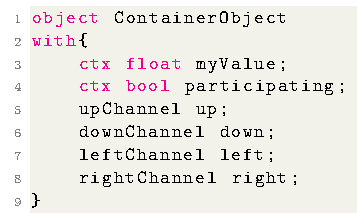
\includegraphics[width=0.3\columnwidth]{imgs/ContainerObject.pdf}
    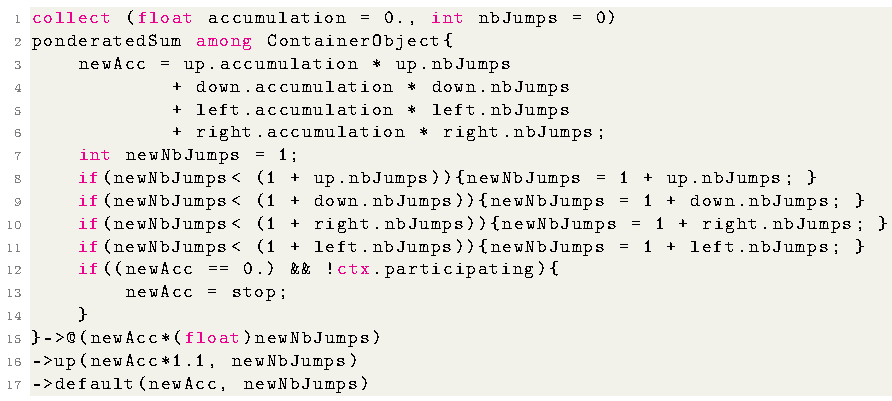
\includegraphics[width=0.65\columnwidth]{imgs/collectivefunctionexample.pdf}
    \caption{An object definition and a collective function to compute a sum of all the functions among the defined object, ponderated by the longest path to a leaf of the tree formed by the configuration used to collect data, putting an emphasis on data propagated via the \emph{up} channel.}\label{collectexample}
\end{figure}

\newpage
\section{Formalisation of Chips modeling semantics}\label{osemantic}

This section is dedicated to mathematically describe the elements of the Chips language that were described earlier in a less formal way. At first, we will define the formalism related the language \emph{functional graphs} (graphs related to the functional block dependencies). Secondly, we will put our focus on the \emph{mapping graphs} (graphs related to the association of functions and virtual objects to physical devices). Finally, we will see how the interconnections between virtual and physical objects define the structures of the datastreams that are profiled and aggragated among the system when using Chips collective primitives.

\subsection{On functional graphs}

The Chips language uses three kinds of primitive types being \emph{integers}, \emph{floating point values} and \emph{booleans}. The sets of all possible values of these types will respectively be denoted \emph{int}, \emph{float} and \emph{bool}, as in current general purpose programming languages. We assume their encoding being implementation dependant so we will not further describe these sets or specific restrictions applied to the operations applied to them.

\paragraph{Notation} We denote the set of Chips types $\mathbb{T}$ as finite arrays of the primitive types \emph{int}, \emph{float} and \emph{bool}:
\begin{align*}
    \mathbb{T} = \{t^i~|~i\in\mathbb{N}^*, t\in\{int,float,bool\}\}
\end{align*}

When mapped by identifiers, types constitute the base element for the construction of function parameter (whether input or output) and variables.

\paragraph{Definition} (Strings) Let $S$ be the set of all possible string sequences that are valid identifiers for vatiables and parameters. From the Chips grammar (Appendix~\ref{grammar}), we see that this set is exactly the language generated from the regular expression \texttt{[a-zA-Z][a-zA-Z0\-9\_]*}, deprived of the set of Chips keywords. 

\paragraph{Remark} (Operational semantics of the imperative aspect of Chips) To assign values to parameters or variables, Chips defines instructions and expressions in a way that is similar to other imperative languages. For concision purposes, we will not detail their semantics and refer to~\cite{plotkin_structural_2004} for examples of equivalent formal interpretation.

\paragraph{Notation} We will denote as $T \in mathbb{T}$ the set of all the values a variable $x \in X^S : T$ can hold, $X^S$ being the set of all defined variables in the scope of the use of this notation.

\paragraph{Notation} For any $X : T^S$, a set of Chips variables, we will denote:
\begin{itemize}
    \item $E[X]$ the set of correctly typed expressions making use of these variables,
    \item $value : E[X] \mapsto T$ the valuation function for a given expression over $X$ into a value of type $T\in\mathbb{T}$ and
    \item $type : E[X] \mapsto \mathbb{T}$ the type deduction function for a correctly typed expression.
\end{itemize}


\paragraph{Definition} (Inputs) Let $\mathbb{I}$ be the set of input parameters for functions. It is made of pairs containing a name $n$ and a value $v$.

\begin{align}
    \mathbb{I} = \{(n,v)~|~n \in S, v \in T\}
\end{align}

\paragraph{Definition} (Outputs) Let $\mathbb{O}$ be the set of output parameters for functions. It is made of pairs containing a name $n$ and an expression $e \in E[X_L]$ over a set of local variables $X_L : T^S$ associated to the function.

\begin{align}
    \mathbb{O} = \{(n,e)~|~n \in S, e \in E[X_L]\}
\end{align}

To facilitate the expression of properties using inputs and outputs, we also define the following functions:
\begin{multicols}{2}
\begin{equation*}
name :
\begin{cases}
(n,v)&\longmapsto n \\
\mathbb{I} &\longmapsto S
\end{cases}
\end{equation*}

\begin{equation*}
type :
\begin{cases}
(n,v)&\longmapsto type(v) \\
\mathbb{I} &\longmapsto \mathbb{T}
\end{cases}
\end{equation*}

\begin{equation*}
value :
\begin{cases}
(n,v)&\longmapsto v \\
\mathbb{I} &\longmapsto T
\end{cases}
\end{equation*}

\begin{equation*}
names :
\begin{cases}
I           &\longmapsto \{name(i)~|~ i \in I\} \\
2^\mathbb{I}&\longmapsto 2^S 
\end{cases}
\end{equation*}

\begin{equation*}
name :
\begin{cases}
(n,e)&\longmapsto n \\
\mathbb{O} &\longmapsto S
\end{cases}
\end{equation*}

\begin{equation*}
type :
\begin{cases}
(n,e)&\longmapsto type(e)\\
\mathbb{O} &\longmapsto \mathbb{T}
\end{cases}
\end{equation*}

\begin{equation*}
value :
\begin{cases}
(n,e)&\longmapsto value(e) \\
\mathbb{O} &\longmapsto T
\end{cases}
\end{equation*}

\begin{equation*}
names :
\begin{cases}
O           &\longmapsto \{name(o)~|~o \in O\} \\
2^\mathbb{O}&\longmapsto 2^S 
\end{cases}
\end{equation*}
\end{multicols}
And finally:
\begin{equation*}
value :
\begin{cases}
n           &\longmapsto 
    \begin{cases}
        \text{if }\exists i \in I, name(i) = n &\text{then } value(i)\\
        \text{if }\exists o \in O, name(o) = n &\text{then } value(o)\\
        \text{if }\exists x \in X, name(x) = n &\text{then } value(x)
    \end{cases} \\
S           &\longmapsto T
\end{cases}
\end{equation*}
With $I$,$O$ and $X$ being respectively the sets of inputs, outputs and variables defined in the scope where the function is used.

For the rest of this paper, we will assume that the names of inputs, outputs and local variables never overlap, even inbetween different functions. This detail is particularly relevant when it comes to describe the operational semantics of our models and is technically easily achievable with character escapement techniques and a correct scope management.

\paragraph{Definition} (Function behavior) One can specify the behavior of functional blocks according to their inputs and outputs using a formalism close to the classic definition of a non-deterministic automaton, enhanced with local variables and a ``readiness'' property explained below. The behavior of a function with (evidently finite) inputs $I \subset \mathbb{I}$ and (also finite) outputs $O \subset \mathbb{O}$ is a tuple\\$B =  (Q,\Sigma,\Delta, X_L, ready)$, where:
\begin{itemize}
    \item $Q$ is a set of states containing exactly $2^{|I|} + 2^{|O|}$ states:
    \begin{itemize}
        \item 2 states representing the initial state $q_{init}$ and the idle state $q_{\emptyset}$,
        \item $2^{|I|}-1$ states, each labelled by a different \textbf{non-empty} unordered set $\iota=\{name(i)~|~i\in I'\subseteq I\}$, which we will write $q_\iota$ for short,
        \item $2^{|O|}-1$ states, each labelled by a different \textbf{non-empty} unordered set $\omega=\{name(o)~|~o\in O'\subseteq O\}$, which we will write $q_\omega$ for short;
    \end{itemize}
    \item $ready\in\{\top,\bot\}$ arbitrarily set;
    \item $X_L$ is a finite set of local data variables that associate an identifier in $S$ to a value of type $T\in\mathbb{T}$;
    \item $\Sigma = \{name(x)~|~x \in I \cup O\}\cup \{\varepsilon\}$ serves as the alphabet of the automaton;
    \item $\Delta$ is the set of all the transition relations $\delta = (q, evt, \pi, g, q')$, such that:
    \begin{itemize}
        \item $(q, q')\in \{(q_I,q_O), (q_{init},q_I), (q_{init},q_\emptyset)\}\\
        \cup \{(q_{\iota},q_{\iota'})~|~\iota\subset\iota'\subseteq \{name(i)~|~i\in I\} \wedge (|\iota| = |\iota'|-1)\}\\
        \cup \{(q_{\omega},q_{\omega'})~|~\{name(o)~|~o\in O\}\supseteq\omega\supset\omega'  \wedge (|\omega'| = |\omega|-1)\}$;
        \item $evt \in \Sigma$ in such way that\\$(q\in \{q_{init},q_{I}\} \Leftrightarrow evt = \varepsilon)\\
        \wedge(\forall \iota \subset I, \forall x \in I, (q, q') = (q_{\iota},q_{\iota\cup\{name(x)\}}) \Rightarrow evt = name(x))\\
        \wedge(\forall \omega \subset O, \forall x \in O, (q, q') = (q_{\omega\cup\{name(x)\}},q_{\omega}) \Rightarrow evt = name(x))$; 
        \item $\pi : I \times X_L \times O \mapsto I \times X_L \times O$ is the process to interpret whenever the transition is applied, ;
        \item $g \in \{\top,\bot\}$ is a guard on the transition equal to $\bot$ iff\\$(ready \wedge (q = q_{init}) \wedge (q' = q_\emptyset)) \vee (\neg ready \wedge (q = q_{init}) \wedge (q' = q_I))$.
    \end{itemize}
\end{itemize}

For any element $\delta = (q, evt, \pi, g, q')$ of $\Delta$, we write $q(\delta)$, $evt(\delta)$, $\pi(\delta)$, $g(\delta)$ and $q'(\delta)$ as the respective components of $\delta$.

\paragraph{Notation} (Substitution) In the remaining of this document, informally, we will write $A[B := C]$ to mean ``the value $A$ for which, in its definition, every instance of the value $B$ is substituted by the value $C$''.

\paragraph{Definition} (Dataflow) A dataflow is a tuple $d=(o,i)$, where:
\begin{itemize}
    \item $o\in\mathbb{O}$,
    \item $i\in\mathbb{I}$ and
    \item $type(o)=type(i)$.
\end{itemize}

\paragraph{Notation} For any dataflow $d = (o,i)$, we note the source of $d$ as $source(d) = o$ and the sink of $d$ as $sink(d) = i$.

\paragraph{Definition} (Functional block) A Chips \textit{functional block} is a tuple\\$f = (B, I, O, I_{default},X_L, init, then, ready)$, where:
\begin{itemize}
    \item $I \subset \mathbb{I}$ and $O\subset\mathbb{O}$ are finite;
    \item $I_{default} \subset \mathbb{I}$ is the set of default values for input of $F$ when they are provided;
    \item $ready = start \vee (\forall i \in I, name(i) \in names(I_{default}))$, with $start$ arbitrarily set to $\top$ or $\bot$;
    \item $X_L \subset S \times T$ is a finite set of local variables;
    \item $init \subset S \times T$ corresponds to the initial values of variables in $X_L$ (defined by a process that we will abstract here);
    \item $then : I \times X_L \mapsto X_L \times O$ is the process that modifies the values of $X_L$ and/or $O$ according to the values of $I$ and the past values of $X_L$;
    \item $B = (Q,\Sigma_f,\Delta, X_L, ready)$ is the function behavior with inputs $I$ and outputs $O$, for which $\Delta$ contains \textbf{exactly} the following transitions:
    \begin{itemize}
        \item $(q_{init}, \varepsilon, X_L:= init; \pi_{init},ready,q_I)$, where \\
        $\pi_{init} \eqdef I := I[\{ i~|~name(i) \in names(I_{default}) \} := I_{default}]$,
        \item $(q_{init}, \varepsilon, X_L:= init; I:=I_{default}, \neg ready, q_\emptyset)$,
        \item $(q_I, \varepsilon, (X_L,O) := then(I,X_L),\top, q_O)$,
        \item Let $D$ be the set of all the instanciated dataflows:\\
        $\forall \delta = (q,evt,\pi,g,q') \in \Delta,\\
        (\forall i\in I, (evt = name(i)) \wedge (\exists (o',i') \in D, name(i') = evt)$\\
        $ \Rightarrow \pi \eqdef value(i) := value(o'))$ and \\
        $(\forall o\in O, (evt = name(o)) \wedge (\exists (o',i') \in D, name(o') = evt)$\\
        $ \Rightarrow \pi \eqdef value(o') := value(o))$.
    \end{itemize}
\end{itemize}

We will call $\mathbb{F}$ the set of possibly definable functional blocks. For this set, we define:
\begin{equation*}
inputs :
\begin{cases}
(B, I, O, I_{default},X_L, init, then, ready)&\longmapsto I \\
\mathbb{F} &\longmapsto \mathbb{I}
\end{cases}
\end{equation*}

\begin{equation*}
outputs :
\begin{cases}
(B, I, O, I_{default},X_L, init, then, ready)&\longmapsto O \\
\mathbb{F} &\longmapsto \mathbb{O}
\end{cases}
\end{equation*}

\paragraph{Definition} (Operational semantics of Chips functional blocks) The operational semantics of a functional block $f = (B, I, O, I_{default},X_L, init, then, ready)$ is given by the LTS $\sigma(f) = (Q \times X_L \times \mathbb{I}, \Sigma, \rightarrow)$ where:
\begin{itemize}
    \item $Q$ is the set of states of the functional block behavior $B$,
    \item $\Sigma$ is the alphabet of that same $B$ and
    \item Let $(q,x)$ be the control state of $f$ with $x\in X_L$, $\rightarrow$ is the minimal transition relation inductively defined by the following rule:
    \begin{equation}
        \begin{split}
            q = q(\delta) \s\s a = evt(\delta)\s\s q' = q(\delta) \s\s g(\delta) = \top \s\s\\
            \cfrac{
                (inputs(f),x',outputs(f)) =  \pi(\delta)(inputs(f),x,outputs(f))
            }
            {
                (q,x) \aoverb{a}{\longrightarrow} (q',x')
            }
        \end{split}
    \end{equation}
    where $a \in \Sigma_f$ is any event that the function $f$ can interpret, i.e.~a writing of an input or a reading of an output.
\end{itemize}

Two particular cases of functional blocks are also worth describing: $CST$ and $buffer$.

\paragraph{Definition} (Constants functional blocks) Chips allows to directly instanciate Constants functional blocks with expressions instead of a definition of functional block plus a functional block instanciation. Their definition is as follow:
\begin{align}
    CST :
    \begin{cases}
        e       & \longmapsto (loop, \emptyset, \{ (\text{"output"}, value(e)) \}, \emptyset ,\emptyset, nop, nop, \top) \\
        E[X]    & \longmapsto \mathbb{F}
    \end{cases}
\end{align}

Where $loop$ is a 1-(initial)state, 1-transition, variable-free function behavior with no updtae process and an alphabet being the singleton $\{\text{"output"}\}$, $nop$ is short for the empty process and $X$ is a set of Chips variables.\\

\paragraph{Definition} (Buffer functional blocks) They are a workaround to let functional blocks \emph{feed} themselves with values they produced. Their definition is as follow:

\begin{align}
    buffer :
    \begin{cases}
        t & \longmapsto (B_t, \{ (\text{"input"}, 0_t, \bot) \}, \{ (\text{"output"}, value(\text{"input"})) \}, \emptyset,\emptyset, nop, nop, \bot) \\
        \mathbb{T}  & \longmapsto \mathbb{F}
    \end{cases}
\end{align}

Composition of functional blocks is achieved by connecting outputs to inputs. Thus defining \emph{dataflows}.

\paragraph{Notation} We write $D[F]$ the set of all the dataflows over a finite set of functional blocks $F \subset \mathbb{F}$.

\paragraph{Definition} (Functional graph) Functional graphs are, as described in Section~\ref{functions}, a fnite directed graph $G_F = (F,D)$ for which vertices $F\subset\mathbb{F}$ (for functions) are instances of functional blocks and edges $D \subset D[F]$ (for dataflows) are the input/output relations between such blocks.
A functional graph $G_F$ holds the following properties:
\begin{itemize}
    \item (input completeness)
    \begin{equation}
        \forall f\in F,\forall i \in inputs(f), \exists d \in D, i = sink(d)
    \end{equation}
    \item (output completeness)
    \begin{equation}
        \forall f\in F,\forall o \in outputs(f), \exists d \in D, o = source(d)
    \end{equation}
    \item (dataflow sources unicity)
    \begin{equation}
        \forall o \in outputs(f),\\(\exists d_1 \in D, source(d_1) = o)\wedge(\exists d_2 \in D, source(d_2) = o) \Rightarrow d_1 = d_2
    \end{equation}
    \item (dataflow sinks unicity)
    \begin{equation}
        \forall i \in inputs(f), \\(\exists d_1 \in D, sink(d_1) = i)\wedge(\exists d_2 \in D, sink(d_2) = i) \Rightarrow d1 = d2
    \end{equation}
\end{itemize}

\paragraph{Definition} (Parallel composition of functional blocks) In our computation model, all functional blocks are to be executed in parallel. Therefore, the operational semantics of each functional block stand simultaneously for every functions. However, the input/output dependecy of functions, modeled by dataflows, imply the synchronization of the different automata of a system. For this purpose, we define the (dataflow related) parallel composition operation
\begin{align}
    \bullet ~//_d~ \bullet : 
    \begin{cases}
        (f_1, f2) &\mapsto f_1[name(source(d)):=d_{label}] \mprod f_2[name(sink(d)):=d_{label}]\\
        \mathbb{F} \times \mathbb{F} &\mapsto \mathbb{F}
    \end{cases}
\end{align}
where: 
\begin{itemize}
    \item $\mprod$ is the mixed (or synchronous) product as defined in~\cite{duboc_mixed_1986},
    \item $d \in D$ is the dataflow that defines which input and output transitions are to be both re-labelled with the same fresh $d$-specific name $d_{label} \in S$.
\end{itemize}

\paragraph{Remark} (On the renaming of our functional blocks labels) When defining our system functional blocks, all the names used are chosen pair-wise distincts. Therefore and undesirably, for any two $f_1, f_2 \in \mathbb{F}$, the mixed product of $f_1$ and $f_2$ is isomorphic to the direct product of $f_1$ and $f_2$. Hence the need to rename the input and output of functional blocks when they are synchronized by a dataflow.

\paragraph{Definition} (Operational semantics of composed functional blocks) 
Let $f_1$ and $f_2$ be any functions of $G_F = (F, D)$ a functional graph. Let $d \in D$ a dataflow for which $source(d) \in outputs(f_1)$ and $sink(d) \in inputs(f_2)$. The semantics of the sub graph formed by the parallel composition of $f_1$ and $f_2$ is simply given by $\sigma(f_1 ~//_d~ f_2)$.\\

\myrule
This hlined section is to be included in the rest of the definition of the operational semantics of the functional blocks.
\myrule

\paragraph{Remark} (Self parallel composition) The above definition holds when the source and sink parameters of a given dataflow $d = (o,i)$ are referencing respectively an output and an input of a same functional block $f = (B, I, O, I_{default},X_L, init, then, ready)$. In such case, the operational semantics of this subgraph of the whole system is given by $\sigma(f ~//_d'~ f')$ where 
\begin{align*}
    (f',d') = (f[I-\{i\}:=r(I-\{i\})][O:=r(O)][X_L:=r(X_L)], d)[i:=r(i)]
\end{align*}
using informally $r$ as the renaming function that chooses new unique names for each variable, parameter or set of such objects.

\paragraph{Definition} (Operational semantics of functional graphs) Let $G_F = (F, D)$ a functional graph achieving input/output completeness and dataflow sources/sinks unicity. The operational semantics of $G_F$ is obtained by the accumulated application of the parallel composition operation on all functional blocks of $G_F$. Let $id \in \mathbb{N}$ be the AAAAAAAAAAAAAAAAAAAAAAAAAAAAAAAAAAA AAAAAAAAAAA AAAAAAAAAAAAAA AAAAAAAAAAAAAAAA Idon't know how to write this formally.
\begin{align}
    \sigma(G_F) = \sigma().
\end{align}

\myrule

\subsubsection{Properties of Chips functional graphs}

In this (subsub)section, we must define:
\begin{itemize}
    \item proof of deadlock freedom for complete graphs with DSS unicity ? 
    \item feedback mechanisms (cyclic graphs)
    \item implicit logical clock cycles description
\end{itemize}

\subsection{On mapping graphs}

In this (sub)section, we must define:
\begin{itemize}
    \item formalism definition for mapping graphs
    \item properties that must hold for correct Chips models
\end{itemize}

\subsubsection{Definitions over mapping graphs}

In this (subsub)section, we must define:
\begin{itemize}
    \item node channels
    \item node contextual data
    \item node types: physical and objects
    \item linking (embedding) functions to nodes
    \item linking (embedding) objects to physicals
    \item plugging channels together
\end{itemize}


\subsubsection{Properties of Chips mapping graphs}

In this (subsub)section, we must define:
\begin{itemize}
    \item configurations (embedding DAGs)
    \item hierarchical composition?
    \item functional graph mapping: check if a configuration can support a logical synchronous program
    \item envisionned properties for model checking (reconfigurability, timing robustness, imprecision robustness, others\ldots?)
\end{itemize}

\subsection{On collective primitives}

In this (sub)section, we must define:
\begin{itemize}
    \item formalism definition for spread and collect
    \item properties enabled by this concept 
\end{itemize}

\subsubsection{Formal definitions for collective primitives}

In this (subsub)section, we must define:
\begin{itemize}
    \item relation with functional graph (safe breaking of DSS unicity)
    \item relation with mapping graph (more particularly nodes and the concept of configuration)
\end{itemize}


\subsubsection{Properties enabled by collective primitives}

In this (subsub)section, we must define:
\begin{itemize}
    \item implementation of control motifs
    \item sensitivity/robustness to reconfigurations
\end{itemize}

\section{Current Chips implementation}
Must talk about:
\begin{itemize}
    \item compilation pipeline
    \item example implemented
\end{itemize}


\section{Current, Future and Related Works}

\subsection{Current and future}

Must talk about:
\begin{itemize}
    \item custom data structures
    \item specification files for domain specific property checking
    \item example implemented for JavaBIP
    \item embeddable code generation
    \item reconfiguration specifications
\end{itemize}

\subsection{Related}
Maybe it should be placed somewhere else in the paper if it is a paper.

Must talk about:
\begin{itemize}
    \item Lustre, Esterel, Signal, Fiacre, VHDL, Amaranth, Eclat, ScaFi, BIP, Tina, Hippo
    \item GenoM specifications for hierarchical models
\end{itemize}


\section{Conclusion}

On a vraiment fait du bon travail, c'est super!

\printbibliography


\newpage
\appendix
\section{Chips grammar}\label{grammar}
The current syntax of the language is defined hereafter in the style of ANTLR4 (BNF enhanced with regular expression elements).
\begin{verbatim}
grammar Chips;
program
    : preamble* system? EOF
    ;
system
    : SYSTEM_KW L_CURL
        s_statement*
      R_CURL
    ;
preamble
    : object_def
    | function_def
    | collective_op_def
    ;
object_def
    : OBJECT_KW IDENTIFIER with_section
    ;
node_mapping
    : HAVING_KW IDENTIFIER AS_KW IDENTIFIER SEMICOL
    ;
function_def
    : l_function_def
    | p_function_def
    ;
collective_op_def
    : c_signature L_CURL
        c_statement*
      R_CURL
      ARROW TARGET_KW L_PARENTH c_expr (COMMA c_expr)* R_PARENTH
      c_output+
    ;
c_output
    : ARROW DEFAULT_KW L_PARENTH c_expr (COMMA c_expr)* R_PARENTH
    | ARROW IDENTIFIER L_PARENTH c_expr (COMMA c_expr)* R_PARENTH
    ;
l_function_def
    : LOGICAL_KW IDENTIFIER L_PARENTH 
        (df_parameter_decl (COMMA df_parameter_decl)*)? R_PARENTH
        init_section
        then_section
        named_output*
    ;
p_function_def
    : PHYSICAL_KW IDENTIFIER L_PARENTH 
        (pdf_parameter_decl (COMMA pdf_parameter_decl)*)? R_PARENTH
        with_section
        init_section
        then_section
        p_named_output*
    ;
c_signature
    : c_keywords L_PARENTH 
        (cdf_defaulted_decl (COMMA cdf_defaulted_decl)*)? R_PARENTH
        IDENTIFIER AMONG_KW IDENTIFIER
    ;
c_keywords
    : SPREAD_KW
    | COLLECT_KW
    ;
with_section
    : WITH_KW L_CURL
        with_statement*
      R_CURL
    ;
with_statement
    : IDENTIFIER IDENTIFIER SEMICOL
    | CTX_KW df_type suffixes IDENTIFIER (ASSIGN expr)? SEMICOL
    | statement
    ;
init_section
    : INIT_KW L_CURL
        (statement)*
      R_CURL
    ;
then_section
    : THEN_KW L_CURL
        (statement)*
      R_CURL
    ;
expr
    : expr0 LT expr
    | expr0 GT expr
    | expr0 LEQ expr
    | expr0 GEQ expr
    | expr0 NEQ expr
    | expr0 EQ  expr
    | expr0 AND expr
    | expr0 OR expr
    | expr0
    ;
expr0
    : expr01 PLUS expr0
    | expr01 MINUS expr0
    | expr01
    ;
expr01
    : MINUS expr1
    | expr1
    ;
expr1
    : expr2 TIMES expr1
    | expr2 DIV expr1
    | expr2 MOD expr1
    | NOT expr2
    | expr2
    ;
expr2
    : INT
    | FLOAT
    | BOOL
    | IDENTIFIER suffixes
    | L_PARENTH expr R_PARENTH
    | CTX_KW PERIOD IDENTIFIER suffixes
    | IDENTIFIER L_PARENTH (expr (COMMA expr)*)? R_PARENTH
    | cast
    ;
cast
    : L_PARENTH df_type R_PARENTH expr
    ;
c_expr
    : c_stopless_expr
    | STOP_KW
    ;
c_stopless_expr
    : c_stopless_expr0 LT c_stopless_expr
    | c_stopless_expr0 GT c_stopless_expr
    | c_stopless_expr0 LEQ c_stopless_expr
    | c_stopless_expr0 GEQ c_stopless_expr
    | c_stopless_expr0 NEQ c_stopless_expr
    | c_stopless_expr0 EQ c_stopless_expr
    | c_stopless_expr0 AND c_stopless_expr
    | c_stopless_expr0 OR c_stopless_expr
    | c_stopless_expr0
    ;
c_stopless_expr0
    : c_stopless_expr01 PLUS c_stopless_expr0
    | c_stopless_expr01 MINUS c_stopless_expr0
    | c_stopless_expr01
    ;
c_stopless_expr01
    : MINUS c_stopless_expr1
    | c_stopless_expr1
    ;
c_stopless_expr1
    : c_stopless_expr2 TIMES c_stopless_expr1
    | c_stopless_expr2 DIV c_stopless_expr1
    | c_stopless_expr2 MOD c_stopless_expr1
    | NOT c_stopless_expr2
    | c_stopless_expr2
    ;
c_stopless_expr2
    : IDENTIFIER c_suffixes
    | INT
    | FLOAT
    | BOOL
    | INPUT_KW
    | CTX_KW PERIOD IDENTIFIER c_suffixes
    | IDENTIFIER PERIOD IDENTIFIER c_suffixes
    | IDENTIFIER L_PARENTH (c_expr (COMMA c_expr)*)? R_PARENTH
    | L_PARENTH c_stopless_expr R_PARENTH
    | c_cast
    ;
c_cast
    : L_PARENTH df_type R_PARENTH c_stopless_expr
    ;
suffixes
    : (L_SQUA expr R_SQUA)*
    ;
c_suffixes
    : (L_SQUA c_stopless_expr R_SQUA)*
    ;
s_suffixable_expr
    : IDENTIFIER
    | IDENTIFIER (L_PARENTH (expr (COMMA expr)*)? R_PARENTH)?
    | block PERIOD IDENTIFIER
    ;
block
    : IDENTIFIER suffixes
    ;
loop_in
    :  IDENTIFIER (L_PARENTH (expr (COMMA expr)*)? R_PARENTH)?
    ;
loop_statement
    : FOREACH_KW IDENTIFIER IN_KW loop_in L_CURL
        statement*
      R_CURL
    ;
c_loop_statement
    : FOREACH_KW IDENTIFIER IN_KW loop_in L_CURL
        c_statement*
      R_CURL
    ;
s_loop_statement
    : FOREACH_KW IDENTIFIER IN_KW s_suffixable_expr L_CURL
        s_statement*
      R_CURL
    ;
if_else_statement
    : if_statement
      ELSE_KW L_CURL
        (statement)*
      R_CURL
    ;
s_if_else_statement
    : s_if_statement
      ELSE_KW L_CURL
        s_statement*
      R_CURL
    ;
c_if_else_statement
    : c_if_statement
      ELSE_KW L_CURL
        c_statement*
      R_CURL
    ;
if_statement
    : IF_KW L_PARENTH expr R_PARENTH L_CURL
        (statement)*
      R_CURL
    ;
s_if_statement
    : IF_KW L_PARENTH expr R_PARENTH L_CURL
        s_statement*
      R_CURL
    ;
c_if_statement
    : IF_KW L_PARENTH c_expr R_PARENTH L_CURL
        c_statement*
      R_CURL
    ;
statement
    : df_type suffixes IDENTIFIER (ASSIGN expr)? SEMICOL
    | IDENTIFIER suffixes ASSIGN expr SEMICOL
    | CTX_KW PERIOD IDENTIFIER suffixes ASSIGN expr SEMICOL
    | loop_statement
    | if_else_statement
    | if_statement
    ;
s_statement
    : IDENTIFIER suffixes IDENTIFIER SEMICOL
    | block PERIOD IDENTIFIER L_PARENTH s_expr R_PARENTH SEMICOL
    | LINK_KW IDENTIFIER suffixes TO_KW IDENTIFIER suffixes SEMICOL
    | s_loop_statement
    | s_if_else_statement
    | s_if_statement
    | statement
    ;
s_expr
    : block PERIOD IDENTIFIER
    | collective_operation block PERIOD IDENTIFIER
    | expr
    ;
collective_operation
    : L_PARENTH IDENTIFIER R_PARENTH
    ;
c_statement
    : cdf_full_declaration SEMICOL
    | IDENTIFIER c_suffixes ASSIGN c_expr SEMICOL
    | CTX_KW PERIOD IDENTIFIER c_suffixes ASSIGN c_expr SEMICOL
    | c_loop_statement
    | c_if_else_statement
    | c_if_statement
    ;
named_output
    : ARROW IDENTIFIER L_PARENTH expr (COMMA expr)* R_PARENTH
    ;
p_named_output
    : ARROW ACTUATOR_KW IDENTIFIER L_PARENTH expr (COMMA expr)* R_PARENTH
    | named_output
    ;
df_parameter_decl
    : df_type suffixes IDENTIFIER (ASSIGN expr)?
    ;
df_type
    : INT_KW
    | FLOAT_KW
    | BOOL_KW
    ;
pdf_parameter_type
    : df_type suffixes
    | SENSOR_KW df_type suffixes
    ;
pdf_parameter_decl
    : pdf_parameter_type IDENTIFIER (ASSIGN expr)?
    ;
cdf_defaulted_decl
    : df_type suffixes IDENTIFIER ASSIGN c_expr
    ;
cdf_full_declaration
    : df_type suffixes IDENTIFIER (ASSIGN c_expr)?
    ;
SYSTEM_KW           : 'system'|'SYSTEM';
INT_KW              : 'int';
FLOAT_KW            : 'float';
BOOL_KW             : 'bool';
LOGICAL_KW          : 'logical';
PHYSICAL_KW         : 'physical';
AS_KW               : 'as';
INIT_KW             : 'init';
THEN_KW             : 'then';
FOREACH_KW          : 'for';
IN_KW               : 'in';
IF_KW               : 'if';
ELSE_KW             : 'else';
TO_KW               : 'to';
LINK_KW             : 'link';
HAVING_KW           : 'having';
INPUT_KW            : 'input';
STOP_KW             : 'stop';
AMONG_KW            : 'among';
SPREAD_KW           : 'spread';
COLLECT_KW          : 'collect';
CTX_KW              : 'ctx';
OBJECT_KW           : 'object';
WITH_KW             : 'with';
BY_KW               : 'by';
TARGET_KW           : '@';
DEFAULT_KW          : 'default';
USING_KW            : 'using';
ACTUATOR_KW         : 'actuator';
SENSOR_KW           : 'sensor';
ARROW               : '->';
PLUS                : '+';
MINUS               : '-';
TIMES               : '*';
DIV                 : '/';
MOD                 : '%';
LT                  : '<';
GT                  : '>';
EQ                  : '==';
LEQ                 : '<=';
GEQ                 : '>=';
NEQ                 : '!=';
AND                 : '&&';
OR                  : '||';
NOT                 : '!';
ASSIGN              : '=';
COMMA               : ',';
SEMICOL             : ';';
L_PARENTH           : '(';
R_PARENTH           : ')';
L_CURL              : '{';
R_CURL              : '}';
L_SQUA              : '[';
R_SQUA              : ']';
COLUMN              : ':';
PERIOD              : '.';
BOOL                : 'true'| 'false';
fragment DIGIT      : [0-9] ;
fragment DOTTED_NUMBER
    : '.'DIGIT+
    | DIGIT+'.'DIGIT*
    ;
fragment ID_START   : [a-zA-Z];
fragment ID_NEXT    : [a-zA-Z0-9_];
FLOAT               : DOTTED_NUMBER;
INT                 : DIGIT+;
IDENTIFIER          : ID_START ID_NEXT*;
NEWLINE : ('\r'? '\n')+ -> skip ;
WS          : [ \t\r]+ -> skip ;
COMMENT     : '//' ~[\r\n]* -> skip ;
\end{verbatim}
\end{document}